\documentclass{article}
\usepackage{pgf}
\usepackage{tikz}
\usepackage{tikz-cd}
\usetikzlibrary{arrows,matrix,calc,intersections, positioning}
\usepackage{amssymb}
\usepackage{amsmath}
\usepackage[utf8]{inputenc}

\begin{document}
\pagestyle{empty}
\begin{tikzcd}
  \mathbb{U}_0 \arrow{r}{\mathrm{d}} & \mathbb{U}_1
  \arrow{r}{\mathrm{d}} & \mathbb{U}_2
\end{tikzcd}


\begin{tikzcd}
  \mathbb{V}_0 \arrow{r}{\mathrm{d}} & \mathbb{V}_1
\end{tikzcd}

\begin{tikzcd}
  \mathbb{U}_0 \otimes \mathbb{V}_0 \arrow{r}{\mathrm{d}} & 
  \mathbb{U}_0 \otimes \mathbb{V}_1 \oplus \mathbb{U}_1 \otimes
  \mathbb{V}_0 \arrow{r}{\mathrm{d}} &
  \mathbb{U}_1 \otimes \mathbb{V}_1 \oplus \mathbb{U}_2 \otimes
  \mathbb{V}_0 \arrow{r}{\mathrm{d}} &
  \mathbb{U}_2 \otimes \mathbb{V}_1
\end{tikzcd}


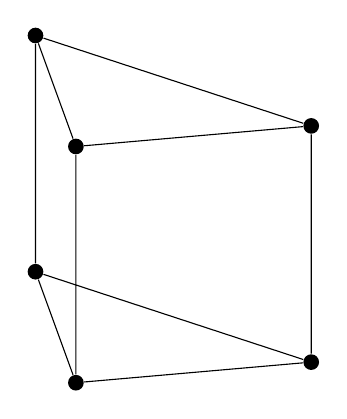
\begin{tikzpicture}[scale=3]

\node [circle, inner sep=2pt, fill=black] (v1) at (0, 0) {};
\node [circle, inner sep=2pt, fill=black] (v2) at ($(0, 0)+(-70:0.5)$) {};
\node [circle, inner sep=2pt, fill=black] (v3) at ($(0, 0)+(-70:0.5) + (5:1)$) {};
\node [circle, inner sep=2pt, fill=black] (v4) at (0, 1) {};
\node [circle, inner sep=2pt, fill=black] (v5) at ($(0, 1)+(-70:0.5)$) {};
\node [circle, inner sep=2pt, fill=black] (v6) at ($(0, 1)+(-70:0.5) + (5:1)$) {};

\draw (v1) -- (v2) -- (v3) -- (v1) -- (v4) -- (v5) -- (v6) -- (v4) (v5) -- (v2) (v3) -- (v6);

\end{tikzpicture}

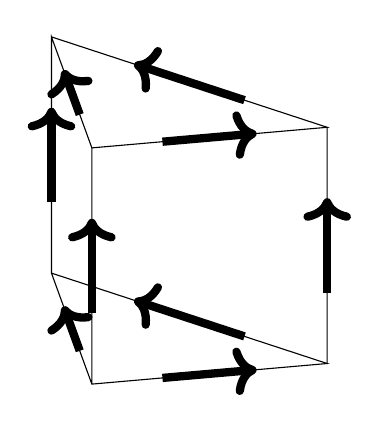
\begin{tikzpicture}[scale=3]

\node  (v1) at (0, 0) {};
\node  (v2) at ($(0, 0)+(-70:0.5)$) {};
\node  (v3) at ($(0, 0)+(-70:0.5) + (5:1)$) {};
\node  (v4) at (0, 1) {};
\node  (v5) at ($(0, 1)+(-70:0.5)$) {};
\node  (v6) at ($(0, 1)+(-70:0.5) + (5:1)$) {};

\draw (v1.center) -- (v2.center) -- (v3.center) -- (v1.center) -- (v4.center) -- (v5.center) -- (v6.center) -- (v4.center) (v5.center) -- (v2.center) (v3.center) -- (v6.center);

\draw[->, line width=3pt] ($(v2)!0.3!(v1)$) -- ($(v2)!0.7!(v1)$); 
\draw[->, line width=3pt] ($(v2)!0.3!(v3)$) -- ($(v2)!0.7!(v3)$); 
\draw[->, line width=3pt] ($(v3)!0.3!(v1)$) -- ($(v3)!0.7!(v1)$); 

\draw[->, line width=3pt] ($(v5)!0.3!(v4)$) -- ($(v5)!0.7!(v4)$); 
\draw[->, line width=3pt] ($(v5)!0.3!(v6)$) -- ($(v5)!0.7!(v6)$); 
\draw[->, line width=3pt] ($(v6)!0.3!(v4)$) -- ($(v6)!0.7!(v4)$); 

\draw[->, line width=3pt] ($(v1)!0.3!(v4)$) -- ($(v1)!0.7!(v4)$);
\draw[->, line width=3pt] ($(v2)!0.3!(v5)$) -- ($(v2)!0.7!(v5)$);
\draw[->, line width=3pt] ($(v3)!0.3!(v6)$) -- ($(v3)!0.7!(v6)$);
\end{tikzpicture}


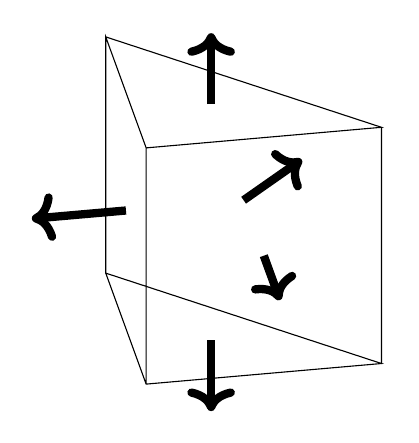
\begin{tikzpicture}[scale=3]

\node  (v1) at (0, 0) {};
\node  (v2) at ($(0, 0)+(-70:0.5)$) {};
\node  (v3) at ($(0, 0)+(-70:0.5) + (5:1)$) {};
\node  (v4) at (0, 1) {};
\node  (v5) at ($(0, 1)+(-70:0.5)$) {};
\node  (v6) at ($(0, 1)+(-70:0.5) + (5:1)$) {};

\draw (v1.center) -- (v2.center) -- (v3.center) -- (v1.center) -- (v4.center) -- (v5.center) -- (v6.center) -- (v4.center) (v5.center) -- (v2.center) (v3.center) -- (v6.center);

\path [name path=v1v5] (v1) -- (v5);
\path [name path=v2v4] (v2) -- (v4);
\path [name intersections={of=v1v5 and v2v4}];
\draw[->, line width=3pt] (intersection-1) -- +(185:0.4);

\path [name path=v2v6] (v2) -- (v6);
\path [name path=v3v5] (v3) -- (v5);
\path [name intersections={of=v2v6 and v3v5}];
\draw[->, line width=3pt] (intersection-1) -- +(-70:0.2);

\path [name path=v3v4] (v3) -- (v4);
\path [name path=v1v6] (v1) -- (v6);
\path [name intersections={of=v3v4 and v1v6}];
\draw[->, line width=3pt] (intersection-1) -- +(35:0.3);

\path [name path=v1mid] (v1) -- ($(v2)!0.5!(v3)$);
\path [name path=v2mid] (v2) -- ($(v3)!0.5!(v1)$);
\path [name intersections={of=v1mid and v2mid}];
\draw[->, line width=3pt] (intersection-1) -- +(0, -0.3);


\path [name path=v4mid] (v4) -- ($(v5)!0.5!(v6)$);
\path [name path=v5mid] (v5) -- ($(v6)!0.5!(v4)$);
\path [name intersections={of=v4mid and v5mid}];
\draw[->, line width=3pt] (intersection-1) -- +(0, 0.3);
\end{tikzpicture}

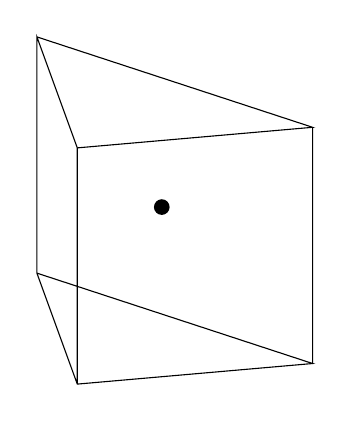
\begin{tikzpicture}[scale=3]

\node  (v1) at (0, 0) {};
\node  (v2) at ($(0, 0)+(-70:0.5)$) {};
\node  (v3) at ($(0, 0)+(-70:0.5) + (5:1)$) {};
\node  (v4) at (0, 1) {};
\node  (v5) at ($(0, 1)+(-70:0.5)$) {};
\node  (v6) at ($(0, 1)+(-70:0.5) + (5:1)$) {};

\draw (v1.center) -- (v2.center) -- (v3.center) -- (v1.center) -- (v4.center) -- (v5.center) -- (v6.center) -- (v4.center) (v5.center) -- (v2.center) (v3.center) -- (v6.center);

\path [name path=v1v5mid] (v1) -- (v6);
\path [name path=v2v4mid] (v2) -- ($(v5)!0.5!(v6)$);
\path [name intersections={of=v1v5mid and v2v4mid}];
\node [circle, fill, black, inner sep=2pt] at (intersection-1) {};
\end{tikzpicture}


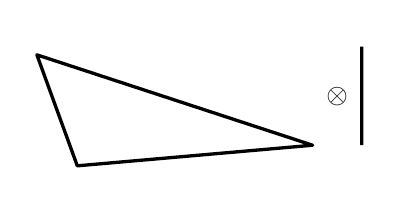
\begin{tikzpicture}[scale=3]
\node  (v1) at (0, 0) {};
\node  (v2) at ($(0, 0)+(-70:0.5)$) {};
\node  (v3) at ($(0, 0)+(-70:0.5) + (5:1)$) {};
\draw[very thick, line join=round] (v1.center) -- (v2.center) -- (v3.center) -- cycle;

\node (v4) [above right=0.5 and 0.05 of v3.south] {$\otimes$};
\node (v5) [right=0.5 of v3.south] {};
\node (v6) at ($(v5) + (0, 0.5)$) {};
\draw[very thick, line join=round] (v5) -- (v6);
\end{tikzpicture}

\newpage
\pgfdeclarelayer{background}
\pgfdeclarelayer{foreground}
\pgfsetlayers{background,main,foreground}
\begin{tikzpicture}[scale=3]
\node [circle, fill, red, inner sep=1.5pt] (v1) at (0, 0) [label=left:$a$] {};
\node [circle, fill, red, inner sep=1.5pt] (v2) at ($(0, 0)+(-70:0.5)$) [] {};
\node [circle, fill, red, inner sep=1.5pt] (v3) at ($(0, 0)+(-70:0.5) + (5:1)$) [label=right:$c$] {};
\node [circle, fill, red, inner sep=1.5pt] (v4) at (0, 0.5) [label=left:$a+1$] {};
\node [circle, fill, red, inner sep=1.5pt] (v5) at ($(0, 0.5)+(-70:0.5)$) [] {};
\node [circle, fill, red, inner sep=1.5pt] (v6) at ($(0, 0.5)+(-70:0.5) + (5:1)$) [label=right:$c+1$]{};

\node [circle, fill, red, inner sep=1.5pt] (v7) at (0, 1) [label=left:$a+2$] {};
\node [circle, fill, red, inner sep=1.5pt] (v8) at ($(0, 1)+(-70:0.5)$) {};
\node [circle, fill, red, inner sep=1.5pt] (v9) at ($(0, 1)+(-70:0.5) + (5:1)$) [label=right:$c+2$] {};

\node [circle, fill, red, inner sep=1.5pt] (v10) at (0, 1.5) [label=left:$a+(n-1)$] {};
\node [circle, fill, red, inner sep=1.5pt] (v11) at ($(0, 1.5)+(-70:0.5)$) {};
\node [circle, fill, red, inner sep=1.5pt] (v12) at ($(0, 1.5)+(-70:0.5) + (5:1)$) [label=right:$c+(n-1)$] {};

\node [circle, fill, red, inner sep=1.5pt] (v13) at (0, 2) [label=left:$a+n$] {};
\node [circle, fill, red, inner sep=1.5pt] (v14) at ($(0, 2)+(-70:0.5)$) {};
\node [circle, fill, red, inner sep=1.5pt] (v15) at ($(0, 2)+(-70:0.5) + (5:1)$) [label=right:$c+n$] {};

\begin{pgfonlayer}{background}
  \draw[very thick, line join=round] (v1.center) -- (v2.center) --
  (v3.center) -- (v1.center) -- (v4.center) -- (v5.center) --
  (v6.center) -- (v4.center) (v5.center) -- (v2.center) (v3.center) --
  (v6.center);

  \draw[very thick, line join=round] (v4.center) -- (v5.center) --
  (v6.center) -- (v4.center) -- (v7.center) -- (v8.center) --
  (v9.center) -- (v7.center) (v8.center) -- (v5.center) (v6.center) --
  (v9.center);

  \draw[very thick, dashed, line join=round] (v7.center) --
  (v10.center) (v8.center) -- (v11.center) (v9.center) --
  (v12.center); \draw[very thick, line join=round] (v10.center) --
  (v11.center) -- (v12.center) -- (v10.center) -- (v13.center) --
  (v14.center) -- (v15.center) -- (v13.center) (v14.center) --
  (v11.center) (v12.center) -- (v15.center);

\end{pgfonlayer}
\end{tikzpicture}

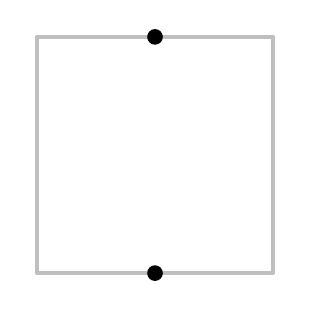
\begin{tikzpicture}[scale=3]
\node  (v1) at (0, 0) {};
\node  (v2) at (1, 0) {};
\node  (v3) at (1, 1) {};
\node  (v4) at (0, 1) {};

\draw[line width=1.5, gray!50, line join=round] (v1.center) -- (v2.center) -- (v3.center) -- (v4.center) -- cycle;

\node [fill, circle, inner sep=2pt, black] at ($(v1)!0.5!(v2)$) {};
\node [fill, circle, inner sep=2pt, black] at ($(v4)!0.5!(v3)$) {};
\end{tikzpicture}


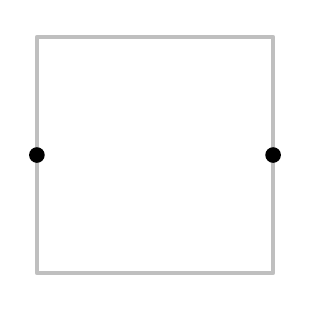
\begin{tikzpicture}[scale=3]
\node  (v1) at (0, 0) {};
\node  (v2) at (1, 0) {};
\node  (v3) at (1, 1) {};
\node  (v4) at (0, 1) {};

\draw[line width=1.5, gray!50, line join=round] (v1.center) -- (v2.center) -- (v3.center) -- (v4.center) -- cycle;

\node [fill, circle, inner sep=2pt, black] at ($(v1)!0.5!(v4)$) {};
\node [fill, circle, inner sep=2pt, black] at ($(v2)!0.5!(v3)$) {};
\end{tikzpicture}


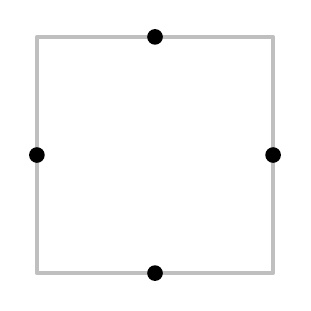
\begin{tikzpicture}[scale=3]
\node  (v1) at (0, 0) {};
\node  (v2) at (1, 0) {};
\node  (v3) at (1, 1) {};
\node  (v4) at (0, 1) {};

\draw[line width=1.5, gray!50, line join=round] (v1.center) -- (v2.center) -- (v3.center) -- (v4.center) -- cycle;

\node [fill, circle, inner sep=2pt, black] at ($(v1)!0.5!(v2)$) {};
\node [fill, circle, inner sep=2pt, black] at ($(v4)!0.5!(v3)$) {};
\node [fill, circle, inner sep=2pt, black] at ($(v1)!0.5!(v4)$) {};
\node [fill, circle, inner sep=2pt, black] at ($(v2)!0.5!(v3)$) {};
\end{tikzpicture}


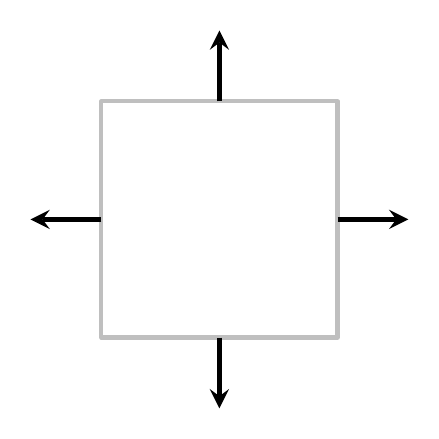
\begin{tikzpicture}[scale=3]
\node  (v1) at (0, 0) {};
\node  (v2) at (1, 0) {};
\node  (v3) at (1, 1) {};
\node  (v4) at (0, 1) {};

\draw[line width=1.5, gray!50, line join=round] (v1.center) -- (v2.center) -- (v3.center) -- (v4.center) -- cycle;

\draw[-stealth, line width=2] ($(v1)!0.5!(v2)$) -- +(0, -0.3);
\draw[-stealth, line width=2] ($(v4)!0.5!(v3)$) -- +(0, 0.3);
\draw[-stealth, line width=2] ($(v1)!0.5!(v4)$) -- +(-0.3, 0);
\draw[-stealth, line width=2] ($(v2)!0.5!(v3)$) -- +(0.3, 0);
\end{tikzpicture}

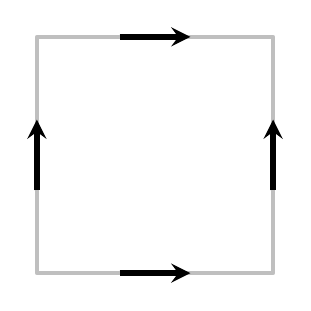
\begin{tikzpicture}[scale=3]
\node  (v1) at (0, 0) {};
\node  (v2) at (1, 0) {};
\node  (v3) at (1, 1) {};
\node  (v4) at (0, 1) {};

\draw[line width=1.5, gray!50, line join=round] (v1.center) -- (v2.center) -- (v3.center) -- (v4.center) -- cycle;

\draw[-stealth, line width=2] ($(v1)!0.35!(v2)$) -- +(0.3, 0);
\draw[-stealth, line width=2] ($(v4)!0.35!(v3)$) -- +(0.3, 0);
\draw[-stealth, line width=2] ($(v1)!0.35!(v4)$) -- +(0, 0.3);
\draw[-stealth, line width=2] ($(v2)!0.35!(v3)$) -- +(0, 0.3);
\end{tikzpicture}

\begin{tikzpicture}[scale=3]
\node  (v1) at (0, 0) {};
\node  (v2) at (1, 0) {};
\node  (v3) at (1, 1) {};
\node  (v4) at (0, 1) {};

\draw[line width=1.5, gray!50, line join=round] (v1.center) -- (v2.center) -- (v3.center) -- (v4.center) -- cycle;
\end{tikzpicture}
\end{document}
